\begin{frame}[fragile]
    \frametitle{Definiciones}
    \begin{alertblock}{Fork:}
        Es una copia exacta de un repositorio, sin embargo tendremos\\
        dos repositorios independientes, con diferente URL que pueden\\
        cada uno evolucionar de forma totalmente aut\'onoma. \\
    \end{alertblock}

    \begin{alertblock}{Repositorio upstream:}
        Es el repositorio original; no podremos hacer ning\'un cambio\\
        directamente sobre este repositorio, ya que no tendremos permisos\\
        de escritura sobre el mismo. Lo que haremos es crear nuestra propia\\
        copia (fork) del mismo.
    \end{alertblock}
\end{frame}

\begin{frame}[fragile]
    \frametitle{Definiciones}
    \begin{alertblock}{Repositorio origin:}
        Es nuestra copia del repositorio que forkeamos alojada en github.\\
        A este repositorio enviaremos los cambios que efectuaremos en nuestro
        \\repositorio local.
    \end{alertblock}

    \begin{alertblock}{Repositorio local:}
        Es el repositorio local que tendremos en nuestra propia estaci\'on 
        de\\trabajo.
    \end{alertblock}
\end{frame}

\begin{frame}[fragile]
    \frametitle{Compartir Repositorio}
    \textbf{1.Hacer un Fork}\\
        Del repositorio upstream, del que haremos copia, de esta forma ya 
        tendremos nuestro repositorio origin.
        \begin{figure}[t]
            \raggedleft
            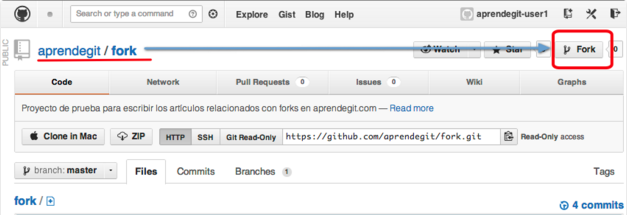
\includegraphics[width=1\textwidth]{Images/6.png}
        \end{figure}
\end{frame}

\begin{frame}[fragile]
    \frametitle{Compartir Repositorio}
    \textbf{2.Clonar repositorio origin en un repositorio local}
    \begin{figure}
        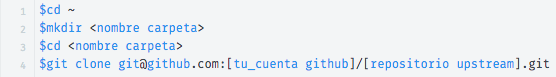
\includegraphics[width=1\textwidth]{Images/7.png}
    \end{figure}

    \textbf{3.Guardar Cambios}
    \begin{figure}
        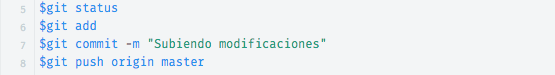
\includegraphics[width=1\textwidth]{Images/8.png}
    \end{figure}
\end{frame}

\begin{frame}[fragile]
    \frametitle{Mantener Repositorios Actualizados}
    Configurar el repositorio upstream como un repositorio remoto (remote)
    vinculado a nuestro repositorio local.Situados en el directorio del 
    repositorio, deberemos ejecutar:
    \begin{figure}
        
\includegraphics[width=1\textwidth]{Images/9.png}
    \end{figure}
    Cuando querramos traer las actualizaciones de upstream, deberemos 
    ejecutar:
    \begin{figure}
        
\includegraphics[width=1\textwidth]{Images/10.png}
    \end{figure}
\end{frame}
